\documentclass[11pt,a4paper]{article}

% -----------------------------------------------------------------------------
% CS6868 Research Mini-Project Report
% -----------------------------------------------------------------------------
\usepackage[utf8]{inputenc}
\usepackage[T1]{fontenc}
\usepackage[margin=0.85in]{geometry}
\usepackage{microtype}
\usepackage{lmodern}
\usepackage{amsmath,amssymb}
\usepackage{graphicx}
\usepackage{booktabs}
\usepackage{array}
\usepackage{enumitem}
\usepackage{xcolor}
\usepackage{listings}
\usepackage{hyperref}
\usepackage[capitalise,noabbrev]{cleveref}

\hypersetup{
  colorlinks=true,
  linkcolor=black,
  citecolor=blue!60!black,
  urlcolor=blue!60!black,
}

\definecolor{codegray}{gray}{0.95}
\lstset{
  basicstyle=\ttfamily\small,
  backgroundcolor=\color{codegray},
  frame=single,
  framesep=4pt,
  breaklines=true,
  columns=fullflexible,
  keepspaces=true,
  showstringspaces=false,
}

\setlist[itemize]{topsep=2pt,itemsep=2pt,leftmargin=1.5em}
\setlist[enumerate]{topsep=2pt,itemsep=2pt,leftmargin=1.5em}

\title{%
  \textbf{CS6868 Research Mini-Project} \\[0.3em]
  \Large Allocation-Conscious Semi-Space Garbage Collection in OxCaml%
}
\author{%
  Aadi Srivastava
  \and
  Aditya Sawant
}
\date{May 2026}

\begin{document}
\maketitle

\begin{abstract}
This project studies whether a semi-space copying garbage collector written in
OxCaml can benefit from zero-allocation and stack-oriented programming features
when compared against a normal OCaml implementation of the same algorithm.  We
implemented a small managed runtime in C with two 128 MiB semi-spaces, explicit
root registration, thread-local root stacks, and a stop-the-world protocol.  The
collector algorithm itself is implemented in five OCaml/OxCaml variants:
ordinary OCaml, zero-allocation OxCaml, C-side scratch-state, persistent-worker
off-heap collection, and a long-lived \texttt{exclave\_} stack-threaded service
loop.  All variants share the same object layout, allocation fast path, root
registry, and benchmark workload.  The benchmark constructs and checks
multi-threaded binary trees across five depths and eight worker counts.  In the
latest run, the normal collector had the lowest aggregate wall-clock mean
(2.133 s) and won 18 of 40 configurations; the closest allocation-free variants
were \texttt{zero} at 2.204 s and \texttt{zero\_stack\_threaded} at 2.220 s.
GC pause means were very close, ranging from 15.20 ms to 16.61 ms.  The main
conclusion is that allocation-free collector code is promising and wins some
configurations, but in this implementation its savings are often offset by FFI
and worker-synchronization overheads.
\end{abstract}

% =============================================================================
\section{Goals}
\label{sec:goals}
% =============================================================================

The goal of this project was to build and evaluate a semi-space copying garbage
collector whose collection algorithm is written in OCaml/OxCaml while the
runtime, heap, root metadata, and stop-the-world protocol are implemented in C.
The project connects to course themes in concurrent runtime design: threads
share heap metadata, mutators must rendezvous at safe points, condition
variables are used to implement stop-the-world coordination, and correctness
depends on preserving root reachability across interleavings.

The project has two implementation goals:
\begin{enumerate}
  \item Build a working C runtime with explicit root tracking, multi-threaded
  allocation, two semi-spaces, and a collector bridge into OCaml/OxCaml.
  \item Implement several collector variants that differ only in how collector
  bookkeeping is represented: ordinary OCaml heap allocation, OxCaml
  zero-allocation, C-side scratch state, persistent worker threads, and
  stack-local service-loop state.
\end{enumerate}

The research question is:

\begin{quote}
\emph{Does a semi-space copying collector written using OxCaml's
zero-allocation and stack-oriented features run faster than a normal OCaml
collector when both share the same C heap, allocation fast path, object layout,
and benchmark workload?}
\end{quote}

A secondary question is when any benefit is large enough to overcome fixed
overheads introduced by FFI calls, noalloc primitives, C-side scratch-state
access, and persistent-worker synchronization.

% =============================================================================
\section{Background}
\label{sec:background}
% =============================================================================

\subsection{Semi-space copying collection}

Semi-space collection divides the heap into two equal regions, usually called
from-space and to-space.  Mutators allocate linearly in from-space using a bump
pointer.  When there is not enough room for the next object, the runtime stops
the mutators, copies all live objects into to-space, updates all roots to point
to the copied locations, swaps the two spaces, and resumes allocation.  Dead
objects are never copied.  This is the classic copying-collector trade-off:
allocation is fast and compaction is automatic, but only half the allocated heap
capacity is available at a time~\cite{wilson1992,gcHandbook}.

Our collector uses Cheney's breadth-first traversal~\cite{cheney1970}.  The
collector maintains two pointers into to-space.  \texttt{free\_ptr} points to
the next free byte after copied objects, and \texttt{scan\_ptr} points to the
next copied object whose fields still need to be scanned.  Initially both point
to the start of to-space.  Copying a root advances \texttt{free\_ptr}.  The
collector then repeatedly scans objects between \texttt{scan\_ptr} and
\texttt{free\_ptr}; any field that points into from-space is copied and the
field is updated.

\begin{lstlisting}[caption={Cheney-style traversal used by every variant.},label={lst:cheney}]
free_ptr = to_space_start
scan_ptr = to_space_start

for root in static_roots and thread_roots:
    root = copy(root, free_ptr)

while scan_ptr < free_ptr:
    header = word_at(scan_ptr)
    for each field in object(scan_ptr):
        field = copy(field, free_ptr)
    scan_ptr += object_size(header)

swap_spaces(free_ptr - to_space_start)
\end{lstlisting}

\subsection{Why zero allocation in the collector?}

A collector runs precisely when an allocation request cannot be satisfied.  If
collector bookkeeping allocates on the managed heap, it adds activity at the
most allocation-sensitive point in execution.  OxCaml provides two relevant
features: zero-allocation annotations, which let the compiler check that
annotated functions do not allocate, and stack/local allocation features such as
\texttt{let mutable}, unboxed tuples, and \texttt{exclave\_} regions
\cite{oxcamlStackIntro,oxcamlStackReference}.  The project tests whether these
features provide a measurable benefit for the collector hot path.

% =============================================================================
\section{Tasks Undertaken}
\label{sec:tasks}
% =============================================================================

\subsection{Runtime and heap implementation}

The C runtime is in \texttt{runtime.c} and \texttt{runtime.h}.  It allocates two
semi-spaces using \texttt{malloc}; each semi-space is 128 MiB.  Allocation is a
simple bump-pointer fast path into \texttt{from\_heap}.  The allocator receives
a payload length and tag, writes a one-word header, initializes payload fields
to tagged zero, advances \texttt{cur\_heap\_ptr}, and returns a pointer to the
object body.

The object representation is intentionally simple and uniform across variants:
\begin{itemize}
  \item Low bit 1 means a tagged integer.
  \item Low bit 0 means either null or a possible heap pointer.
  \item A heap pointer points to the object body; the header is one word before
  the body.
  \item The header is encoded as \texttt{(total\_words << 10) | tag}.
  \item A forwarded object has old header 0 and stores the new body address in
  old field 0.
\end{itemize}

This layout makes the copy operation cheap: check whether a word is a
from-space pointer, check whether it was already forwarded, copy
\texttt{total\_words} words into to-space, install a forwarding marker, and
return the new body address.

\begin{table}[h]
\centering
\small
\begin{tabular}{@{}p{0.28\linewidth}p{0.64\linewidth}@{}}
\toprule
\textbf{File} & \textbf{Responsibility} \\
\midrule
\texttt{runtime.h} & Public C runtime interface, object-tagging macros, root
frame macros, thread registry declarations, STW state definition. \\
\texttt{runtime.c} & Heap allocation, two semi-spaces, root stack operations,
thread spawn/join wrappers, STW safe-point protocol. \\
\texttt{gc\_bridge.c} & OCaml runtime startup, noalloc primitive definitions,
collector callback dispatch, persistent GC worker, pause logging. \\
\texttt{gc\_prims.ml} & Shared OxCaml external declarations for heap access,
root iteration, off-heap state, and service-loop hooks. \\
\texttt{gc\_*.ml} & Five collector variants implementing the same copying
algorithm with different bookkeeping strategies. \\
\texttt{tests/binary\_tree\_multithreaded.c} & Correctness and performance
stress workload used by every binary. \\
\bottomrule
\end{tabular}
\caption{Main implementation files and their roles.}
\label{tab:filemap}
\end{table}

Several invariants are shared by all collector variants.  First, an object body
address is stable until the next collection, and any body pointer can recover
its header by subtracting one word.  Second, only words that are non-null,
low-bit-zero, and inside from-space are treated as candidate pointers.  Third,
after an object is copied, the old header is zero; this makes forwarding tests
constant-time.  Fourth, \texttt{cur\_heap\_ptr} is an offset in bytes, not a
raw pointer, so swapping \texttt{from\_heap} and \texttt{to\_heap} only requires
storing the number of used bytes in the new from-space.

\subsection{Explicit root tracking}

The benchmark is written in C, so roots are explicitly registered.  Each thread
has a thread-local root stack, frame-size stack, current frame index, and
return-value root.  \texttt{make\_root} pushes the address of a local pointer
variable into the root stack; \texttt{make\_return\_root} preserves a value
across a return; \texttt{alloc\_free\_new\_frame} and
\texttt{alloc\_free\_return\_with\_val} implement frame entry and exit.

Thread-local root state is exposed to the collector through a global registry:
each active thread records the address of its root stack, stack index, return
slot, and active flag.  Static roots are stored in a separate bounded array.
During collection the OCaml/OxCaml collector iterates through the registry using
noalloc C primitives and updates roots in place.

\subsection{Stop-the-world synchronization}

The stop-the-world protocol uses one mutex and three condition variables in
\texttt{STW\_State}.  Allocation overflow is the main safe point, and
\texttt{poll\_for\_gc} provides an additional safe point used around blocking
operations such as joins.  When a mutator requests GC, it increments the stopped
count and waits until all active mutators have reached a safe point.  Once the
world has stopped, the allocator drops the STW lock and calls
\texttt{run\_collection}.  Dropping the lock is safe because all mutators are
parked; it also prevents the OCaml collector from contending with the STW lock
while reading the root registry.

Thread spawning and joining update \texttt{num\_threads}.  The joining thread is
temporarily removed from the live count while blocked in \texttt{pthread\_join};
otherwise, a GC requested while the joiner sleeps could wait for a thread that
cannot reach a safe point.

The STW protocol is conservative: while collection runs, no mutator writes heap
fields or root variables.  That is why the collector can update C root variables
directly through raw addresses.  The collector also runs outside the STW mutex;
this avoids deadlock with helper functions and keeps the STW lock focused on
coordination rather than on the full traversal time.  The design assumes one
collector at a time, which is enforced by the allocation path that requests GC
while holding the STW mutex.

\subsection{C--OxCaml bridge}

\texttt{gc\_bridge.c} is the FFI boundary.  It starts the OCaml runtime,
initializes OCaml systhreads, registers callbacks, exposes noalloc primitives,
and dispatches to the selected collector variant.  It deliberately does not
include \texttt{runtime.h}, because both OCaml headers and our runtime define
names such as \texttt{Field}; instead, it re-declares only the runtime symbols
that it needs.

The bridge provides primitives such as:
\begin{itemize}
  \item heap bounds: \texttt{from\_space\_start}, \texttt{from\_space\_end},
  \texttt{to\_space\_start};
  \item raw word access: \texttt{word\_at}, \texttt{set\_word\_at},
  \texttt{memcpy\_words};
  \item root iteration: static root count/address and per-thread root-stack
  accessors;
  \item finalization: \texttt{swap\_spaces};
  \item off-heap scratch state for variants 3 and 4; and
  \item service-loop wait/done hooks for variant 5.
\end{itemize}

It also records per-collection pause times using \texttt{clock\_gettime}.  Each
collection appends a row to \texttt{benchmarking/gc\_pauses\_<variant>.csv}.
This logging is useful for analysis, but it is also a limitation because the
current implementation opens and closes the pause file after each collection,
which adds wall-clock overhead outside the timed pause interval.

There are three bridge dispatch modes.  In the synchronous mode, used by
\texttt{normal}, \texttt{zero}, and \texttt{zero\_offheap}, the mutator thread
that requested collection temporarily enters the OCaml runtime and calls the
registered \texttt{gc\_collect} callback.  In the persistent-worker mode, used
by \texttt{zero\_offheap\_threaded}, a worker thread registers with the OCaml
runtime once and then waits on a command condition variable.  In the
stack-threaded mode, used by \texttt{zero\_stack\_threaded}, the worker calls a
registered \texttt{gc\_service\_run} callback once; the OCaml function itself
contains the infinite service loop and waits through noalloc service hooks.
This distinction matters because variant 5 is not merely a callback on a worker
thread: it is a long-lived OxCaml frame designed to keep collector state in the
service function.

\subsection{Collector variants}

All variants implement the same traversal and root scan.  Their differences are
only in collector bookkeeping and invocation strategy.  We designed the five
variants as a sequence: each variant answers one question left open by the
previous one, while preserving the same object representation, root scanning
order, forwarding scheme, and benchmark workload.

\paragraph{Variant 1: \texttt{normal}.}
\texttt{gc\_normal.ml} is the baseline.  It uses ordinary OCaml refs for
\texttt{free\_ptr} and \texttt{scan\_ptr}.  The \texttt{copy} helper returns an
ordinary boxed pair \texttt{(new\_value, new\_free\_ptr)}.  This version is the
clearest reference implementation and intentionally has no zero-allocation
annotation.

The baseline is important because it is not a deliberately slow collector.  It
uses the same C heap, noalloc memory-access stubs, root registry, forwarding
layout, and STW protocol as every other variant.  Its only disadvantage is
ordinary OCaml bookkeeping in the collector.  This makes it the right reference
point for the project question: if the normal collector is already competitive,
then avoiding OCaml allocations in the collector hot path must produce a real
enough saving to overcome all extra mechanisms introduced by later variants.

The transition from variant 1 to variant 2 isolates one cost: boxed collector
bookkeeping.  In the normal collector, \texttt{copy} communicates two results by
allocating a pair, and mutable refs store scan/free state.  Variant 2 keeps the
same synchronous callback structure but rewrites this bookkeeping using OxCaml
features.

\paragraph{Variant 2: \texttt{zero}.}
\texttt{gc.ml} rewrites the same algorithm using OxCaml \texttt{let mutable}
variables and an unboxed tuple return:
\begin{lstlisting}[caption={Allocation-free copy return shape.},label={lst:unboxed}]
let[@zero_alloc] copy v free_ptr : #(int * int) =
  ...
  #(new_body_addr, free_ptr + bytes)
\end{lstlisting}
The \texttt{[@zero\_alloc]} annotations enforce that the collector hot path does
not allocate OCaml heap objects.

This variant uses \texttt{let mutable free\_ptr} and \texttt{let mutable
scan\_ptr} rather than OCaml refs.  The copy helper returns
\texttt{\#(value, free\_ptr)} so no boxed pair is allocated on the OCaml heap.
The function bodies are annotated with \texttt{[@zero\_alloc]}, and small helper
functions in \texttt{gc\_prims.ml}, such as \texttt{header\_total\_words} and
\texttt{is\_forwarded}, are also marked zero-allocation and inlined so the
checker can prove the property.  The code therefore tests the most direct
OxCaml hypothesis: can we remove collector-local allocation while leaving the
runtime and invocation path unchanged?

The transition from variant 2 to variant 3 asks whether there is still too much
OCaml-side state in the collector.  Variant 2 keeps the free and scan pointers
as stack locals inside one collection invocation.  Variant 3 moves this scratch
state outside the OCaml heap entirely, into C globals accessed through noalloc
primitives.

\paragraph{Variant 3: \texttt{zero\_offheap}.}
\texttt{gc\_zero\_offheap.ml} removes OCaml-side persistent scratch state for
the collector.  \texttt{free\_ptr} and \texttt{scan\_ptr} live in C globals and
are accessed through noalloc get/set primitives.  This avoids OCaml refs and
unboxed pair returns, but it increases FFI traffic.

In this variant, copying an object reads \texttt{g\_free\_ptr}, copies the
object to that address, installs the forwarding marker, and writes back the
advanced \texttt{g\_free\_ptr}.  During the Cheney walk, the OCaml loop keeps a
local view of \texttt{scan\_ptr} but refreshes \texttt{free\_ptr} after field
copies because \texttt{copy\_into} may have advanced the C-side free pointer.
This design removes OCaml allocation from the collector state, but it also
adds more C boundary crossings than variant 2.

The benchmark results suggest that this trade-off is unfavorable for the
current workload: \texttt{zero\_offheap} has the highest aggregate mean and no
configuration wins in the latest grid.  That does not mean off-heap state is
always bad; it means the cost of frequent noalloc get/set calls is visible when
the state is touched in the inner copy path.

The transition from variant 3 to variant 4 therefore targets invocation cost
rather than state representation.  If C-side scratch state is going to be used,
we also want to reduce repeated runtime entry and C-thread registration costs.
Variant 4 does this with a persistent OCaml-aware worker thread.

\paragraph{Variant 4: \texttt{zero\_offheap\_threaded}.}
\texttt{gc\_zero\_offheap\_threaded.ml} uses the same collector algorithm and
off-heap scratch state as variant 3, but \texttt{gc\_bridge.c} invokes it from a
persistent OCaml-aware worker thread.  The worker sleeps on a condition
variable, wakes for collection, runs \texttt{gc\_collect}, signals completion,
and sleeps again.

Most of the change for variant 4 is in \texttt{gc\_bridge.c}, not in the OCaml
collector file.  At runtime initialization, \texttt{start\_gc\_service} creates
a worker.  The worker calls \texttt{caml\_c\_thread\_register}, acquires the
OCaml runtime lock when needed, and then waits on \texttt{gc\_cmd\_cond}.  When
\texttt{run\_collection} is called by the stopped mutator, it signals the
worker and waits on \texttt{gc\_done\_cond}.  The worker runs the same
\texttt{gc\_collect} callback and reports completion.

This variant separates two effects.  It keeps variant 3's C-side scratch state,
but removes repeated setup for entering OCaml from arbitrary C threads.  It
also introduces a new overhead: condition-variable handoff between the mutator
that requested GC and the worker that performs GC.  In the latest benchmark it
wins six configurations, so the persistent worker helps in selected cases, but
the handoff cost prevents a consistent win.

The transition from variant 4 to variant 5 is the main stack-allocation
experiment.  Variant 4 still calls a collection function once per GC.  Variant
5 instead calls into OCaml once and stays there in a long-lived service loop,
so the collector can use the worker's persistent OxCaml stack frame.

\paragraph{Variant 5: \texttt{zero\_stack\_threaded}.}
\texttt{gc\_stack\_threaded.ml} runs a long-lived OxCaml service loop registered
as \texttt{gc\_service\_run}.  The function enters an \texttt{exclave\_} region,
then loops forever: wait for a service command, collect, call
\texttt{service\_done}.  Within each collection, \texttt{free\_ptr} and
\texttt{scan\_ptr} are \texttt{let mutable} stack locals and the copy helper
returns an unboxed tuple.  We intentionally avoided general-purpose collector
optimizations such as skipping unchanged \texttt{set\_word\_at} calls, because
those could also be applied to the normal baseline and would make the comparison
less focused on allocation-free programming.

The key difference from variant 4 is that the OCaml worker does not repeatedly
enter and leave a collector callback.  It calls \texttt{service\_run} once, and
that function contains the infinite command loop:
\begin{lstlisting}[caption={Shape of the stack-threaded service loop.},label={lst:service}]
let[@zero_alloc] service_run () = exclave_
  let[@inline always] copy_into v free_ptr : #(int * int) = ...
  while true do
    service_wait ();
    let mutable free_ptr = to_space_start () in
    let mutable scan_ptr = free_ptr in
    ... root scan and Cheney walk ...
    swap_spaces (free_ptr - to_start);
    service_done ()
  done
\end{lstlisting}

\texttt{service\_wait} releases the OCaml runtime lock while blocked on the C
condition variable, then reacquires it before returning to OxCaml code.  This
keeps the worker asleep without monopolizing the runtime lock.  The use of
\texttt{exclave\_} and \texttt{let mutable} expresses the intended allocation
discipline: collector state lives in the service frame and per-collection stack
locals, while \texttt{copy\_into} communicates the updated free pointer using an
unboxed tuple.  This variant is the closest allocation-free design on aggregate
after \texttt{zero}; it wins six configurations and is especially competitive
at depth 14, but it still pays worker wake/sleep synchronization.

The sequence of variants therefore gives a clean progression:
\begin{enumerate}
  \item establish a normal OCaml baseline;
  \item remove boxed collector-local allocation;
  \item move scratch state outside OCaml values;
  \item amortize callback setup with a persistent worker; and
  \item use a long-lived OxCaml service frame for stack-local collector state.
\end{enumerate}

\begin{table}[h]
\centering
\small
\begin{tabular}{@{}p{0.22\linewidth}p{0.23\linewidth}p{0.42\linewidth}@{}}
\toprule
\textbf{Variant} & \textbf{Invocation} & \textbf{Bookkeeping representation} \\
\midrule
\texttt{normal} & synchronous callback & OCaml refs and boxed pair returns. \\
\texttt{zero} & synchronous callback & \texttt{let mutable} locals and unboxed
\texttt{\#(int * int)} returns. \\
\texttt{zero\_offheap} & synchronous callback & C globals for
\texttt{free\_ptr}/\texttt{scan\_ptr}; noalloc get/set stubs. \\
\texttt{zero\_offheap\_threaded} & persistent worker callback & Same C-side
scratch state as \texttt{zero\_offheap}. \\
\texttt{zero\_stack\_threaded} & long-lived service loop & \texttt{exclave\_}
service frame; per-collection \texttt{let mutable} stack locals. \\
\bottomrule
\end{tabular}
\caption{How the variants differ while preserving the same copying algorithm.}
\label{tab:variants}
\end{table}

\subsection{Build and benchmark tooling}

The Makefile builds one binary per variant, for example
\texttt{bin/bench\_zero\_stack\_threaded}.  The OCaml code is compiled into a
complete native object with \texttt{ocamlopt -output-complete-obj}; the C
runtime, bridge, and benchmark are then linked with \texttt{libasmrun.a} and
\texttt{libthreadsnat\_stubs.a}.  \texttt{benchmarking/bench.sh} builds all
variants and runs the depth/thread grid.  \texttt{benchmarking/summarize.py}
prints aggregate statistics, and \texttt{benchmarking/plot\_benchmark.py}
generates the plots used in this report.

\subsection{Testing and verification}

Correctness testing has two layers.  First, small smoke tests verify that each
binary starts, initializes the runtime, builds trees, performs collections, and
prints \texttt{done}.  Second, the main benchmark validates semantic
correctness by checking node counts for stretch trees, temporary trees, and
long-lived trees.  For a fixed input, the \texttt{[T]} checksum lines must match
across all five variants.  We compare sorted checksum lines because worker
threads print in nondeterministic order.

This testing caught important issues.  The initial build failed to link because
the OCaml C-thread registration functions require
\texttt{libthreadsnat\_stubs.a}.  The zero-allocation checker also rejected
helpers until the pure header helpers were marked \texttt{[@zero\_alloc]} and
\texttt{[@inline always]}.  A later runtime crash in the persistent-worker
variant was traced to OCaml systhreads not being initialized before
\texttt{caml\_c\_thread\_register}; the bridge now calls
\texttt{caml\_thread\_initialize} during startup.

The benchmark is also a regression test for the root protocol.  The recursive
\texttt{make} function creates left and right subtrees and then allocates a
parent object; without explicit roots, a GC between these allocations could
move or reclaim a subtree while the C local variable still holds an old address.
Similarly, \texttt{mk\_data} returns an allocated object through
\texttt{make\_return\_root}.  These cases are intentionally present so that
missed roots show up as checksum mismatches or crashes.

% =============================================================================
\section{Evaluation}
\label{sec:evaluation}
% =============================================================================

\subsection{Experimental setup}

The benchmark is \texttt{tests/binary\_tree\_multithreaded.c}.  Each worker
builds a stretch tree, a long-lived tree, and many temporary balanced trees.
The data payload for each leaf allocates an eight-word object, so the workload
exercises both pointer fields and tagged integer fields.  Each worker computes
node-count checksums after allocation and collection.  The benchmark stresses:
root updates after copying, return-root survival across function returns,
long-lived reachability, and pointer validity after mutators resume.

The latest grid used:
\begin{itemize}
  \item tree depths: 10, 11, 12, 13, 14;
  \item worker threads: 1 through 8;
  \item variants: \texttt{normal}, \texttt{zero}, \texttt{zero\_offheap},
  \texttt{zero\_offheap\_threaded}, and \texttt{zero\_stack\_threaded};
  \item one run per configuration; and
  \item metrics: wall-clock elapsed seconds and per-collection pause time.
\end{itemize}

There are 40 configurations per variant and 200 benchmark runs in total.  The
machine was the development WSL/Linux environment used for the project.  Because
there is one run per configuration, the results should be read directionally:
thread scheduling, filesystem effects, and pause logging can all add noise.

\subsection{Aggregate wall-clock results}

\begin{table}[h]
\centering
\small
\begin{tabular}{@{}lrr@{}}
\toprule
\textbf{Variant} & \textbf{Mean wall time (s)} & \textbf{Fastest configs} \\
\midrule
\texttt{normal} & 2.133 & 18 / 40 \\
\texttt{zero} & 2.204 & 10 / 40 \\
\texttt{zero\_offheap} & 2.348 & 0 / 40 \\
\texttt{zero\_offheap\_threaded} & 2.231 & 6 / 40 \\
\texttt{zero\_stack\_threaded} & 2.220 & 6 / 40 \\
\bottomrule
\end{tabular}
\caption{Aggregate mean wall-clock time and win count across the latest 40
configurations per variant.}
\label{tab:wall}
\end{table}

\begin{figure}[h]
  \centering
  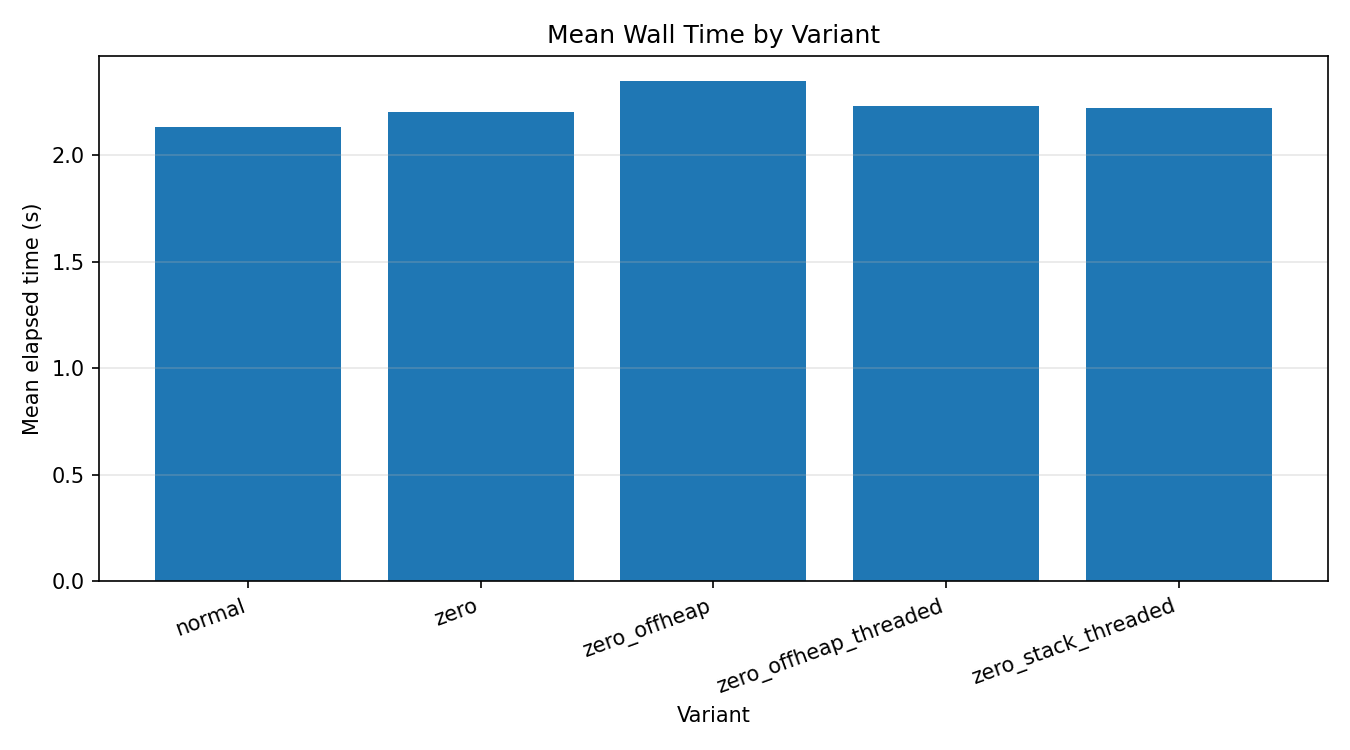
\includegraphics[width=0.73\linewidth]{figures/meanwall.png}
  \caption{Mean wall-clock time by variant. Lower is better.}
  \label{fig:wall}
\end{figure}

\Cref{tab:wall,fig:wall} show that the normal OCaml collector is the aggregate
winner in this run.  This was not the result we initially expected.  The
\texttt{zero} and \texttt{zero\_stack\_threaded} variants are close, but the
savings from removing OCaml heap allocation in collector bookkeeping were not
large enough to dominate the fixed overheads.  The off-heap scratch-state
variant is slower on average, suggesting that extra noalloc FFI calls can cost
more than the OCaml allocation they replace for this workload.

\subsection{Scaling with threads}

\begin{figure}[h]
  \centering
  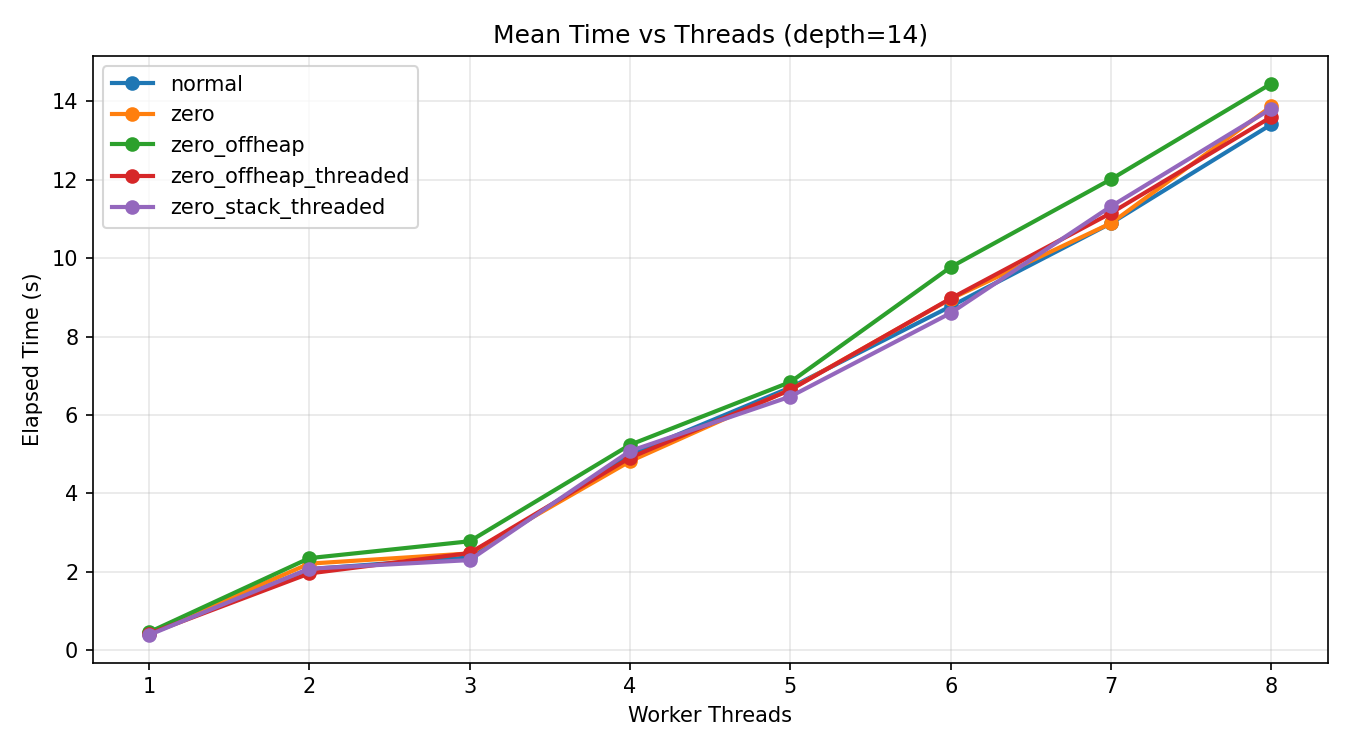
\includegraphics[width=0.82\linewidth]{figures/depth14.png}
  \caption{Elapsed time vs. worker threads at depth 14.}
  \label{fig:depth14}
\end{figure}

\Cref{fig:depth14} shows the largest-depth configuration.  At depth 14, the
stack-threaded service loop is fastest at several thread counts, but normal is
fastest at eight threads.  This illustrates the main pattern: allocation-free
structure can help in pockets, but no variant dominates across the grid.  The
persistent-worker variants are especially sensitive to condition-variable
handoff costs; as contention increases, those costs can erase the benefit of
keeping collector state off the OCaml heap or on the OxCaml stack.

\begin{figure}[h]
  \centering
  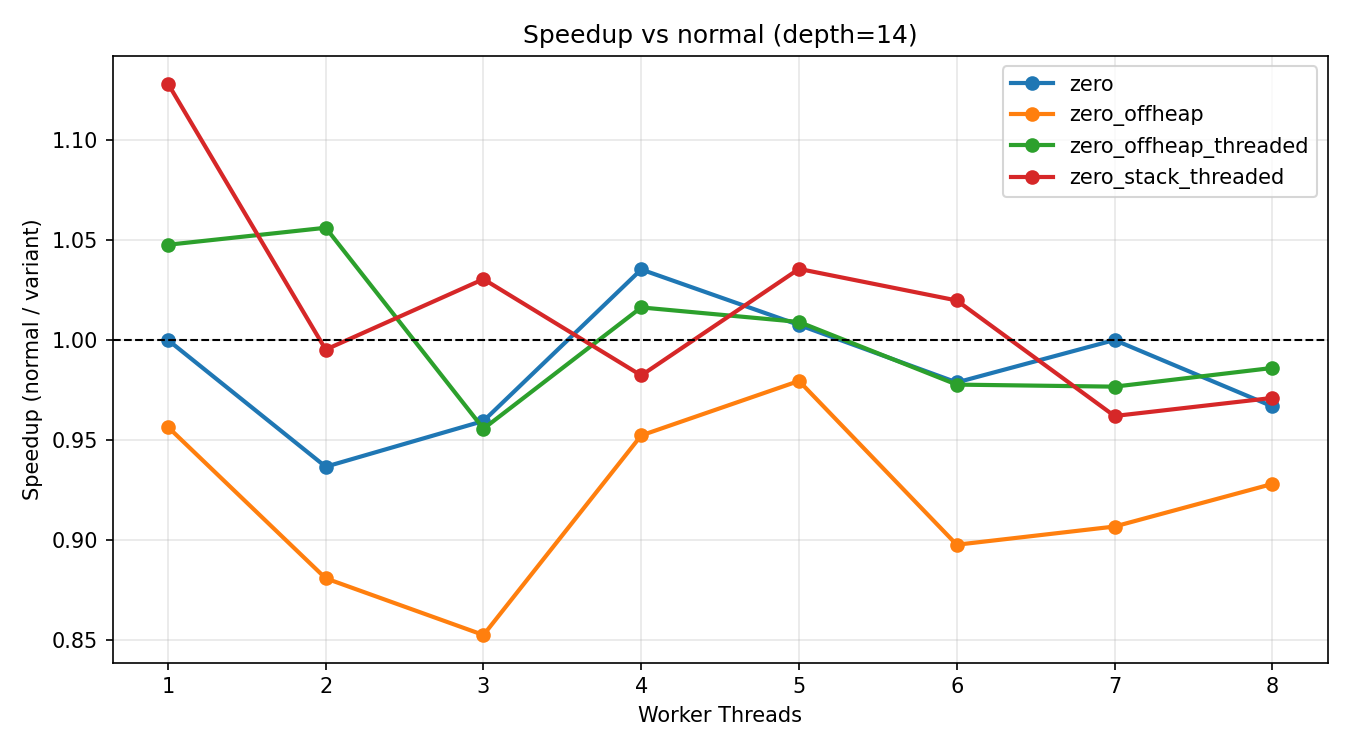
\includegraphics[width=0.82\linewidth]{figures/speedup14.png}
  \caption{Speedup relative to \texttt{normal} at depth 14. A value above 1.0
  means the variant beats the normal baseline.}
  \label{fig:speedup}
\end{figure}

The speedup plot in \cref{fig:speedup} makes the same point from another angle.
Several allocation-free points exceed parity, but the lines cross repeatedly.
This implies that the effect size is small enough for scheduling and runtime
coordination overheads to matter.  The conclusion is not that allocation-free
collector code is useless; rather, it is not a free win under this particular
runtime, workload, and heap size.

\subsection{Pause-time results}

\begin{table}[h]
\centering
\small
\begin{tabular}{@{}lrrr@{}}
\toprule
\textbf{Variant} & \textbf{Mean pause (ms)} & \textbf{p50 (ms)} & \textbf{p99 (ms)} \\
\midrule
\texttt{normal} & 15.20 & 13.81 & 39.53 \\
\texttt{zero} & 15.34 & 14.07 & 40.98 \\
\texttt{zero\_offheap} & 16.61 & 15.20 & 47.09 \\
\texttt{zero\_offheap\_threaded} & 15.97 & 14.73 & 43.71 \\
\texttt{zero\_stack\_threaded} & 15.40 & 14.59 & 41.93 \\
\bottomrule
\end{tabular}
\caption{GC pause statistics across 160 measured collections per variant.}
\label{tab:pause}
\end{table}

\begin{figure}[h]
  \centering
  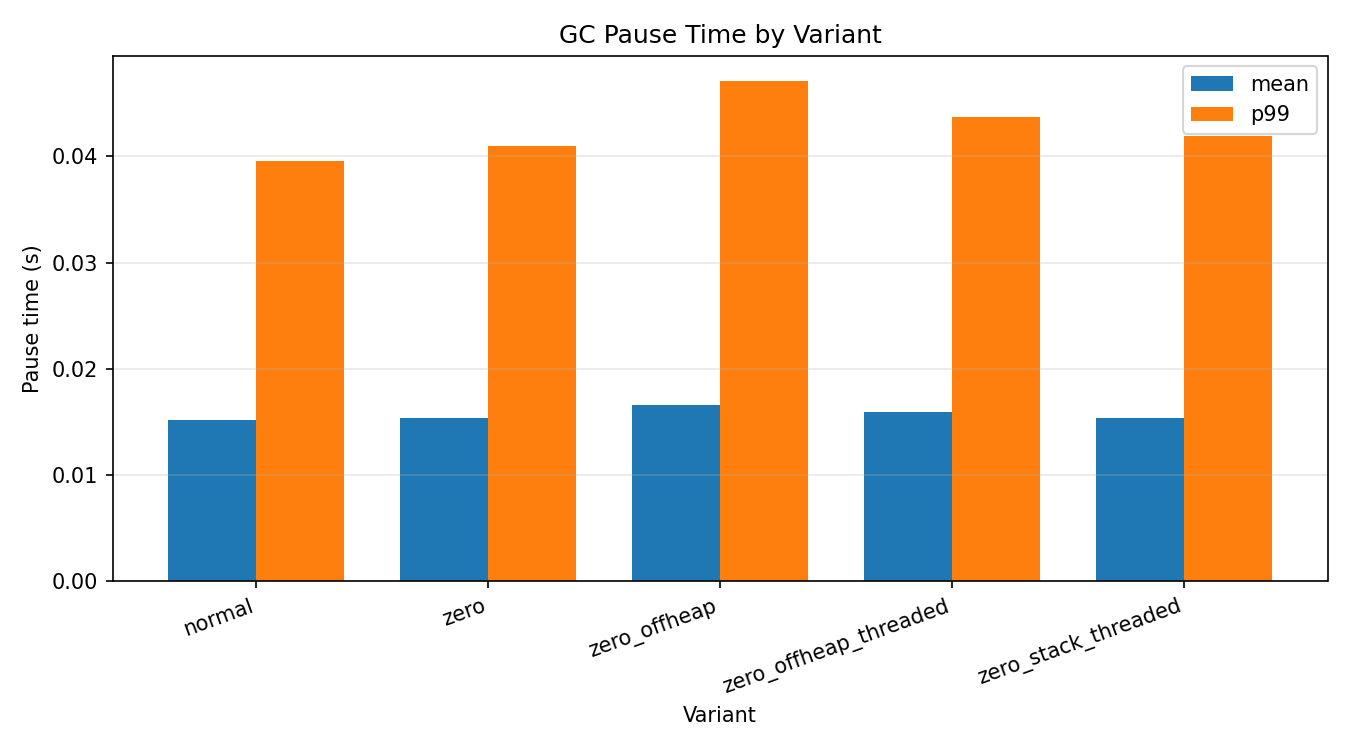
\includegraphics[width=0.75\linewidth]{figures/gcpauses.png}
  \caption{Mean and p99 GC pause times. Lower is better.}
  \label{fig:pause}
\end{figure}

Pause times are close across variants.  The normal collector has the lowest mean
pause, while \texttt{zero\_stack\_threaded} is close.  \texttt{zero\_offheap}
has the highest mean and p99 pause.  The pause results reinforce the wall-clock
interpretation: the algorithmic work of copying live objects dominates, and the
allocation-free variants do not remove enough overhead to clearly reduce pause
time.  The off-heap design also pays for extra FFI transitions in the copy loop.

\subsection{Discussion}

The most important result is negative but useful: simply making collector code
allocation-free does not guarantee faster execution.  The baseline collector's
OCaml allocations are short-lived and may be cheap relative to object traversal,
raw memory copying, C/OCaml boundary crossings, and synchronization.  In
addition, every variant already keeps the mutator heap and root registry in C,
so the normal collector is not an intentionally inefficient baseline.

The \texttt{zero} variant is the cleanest test of zero-allocation alone.  Its
mean is only about 3.3\% slower than normal, and it wins 10 configurations.
This suggests that zero-allocation restructuring is viable, but the benefit is
small.  The \texttt{zero\_stack\_threaded} variant is the most faithful test of
OxCaml stack-local service-loop state.  It wins six configurations and is close
to normal, but its worker synchronization cost remains visible.

The evaluation has clear limitations.  First, each configuration was run once.
Second, the heap is large enough that there are only 160 measured collections
per variant, so wall-clock time includes substantial mutator work.  Third,
pause logging currently performs file I/O after each collection.  Fourth, we
measure time but not copied bytes, live-set size, or FFI-call counts.  These
metrics would help separate collector improvements from workload and scheduling
effects.

% =============================================================================
\section{Reflection on the Use of LLMs}
\label{sec:llm}
% =============================================================================

\paragraph{Tools and models used.}
We used Codex, GPT-5.5, and Gemini Pro through GitHub Copilot during different
parts of the project.  The tools were mainly used for code navigation, basic C
syntax and build checks, debugging compiler and linker errors, drafting
benchmarking and plotting scripts, summarising benchmark results, and improving
documentation.  For OxCaml-specific work, we also supplied additional context
from the official OxCaml documentation and OxCaml-focused skill notes inspired
by Anil Madhavapeddy's discussion of zero-allocation OxCaml systems
\cite{madhavapeddyOxCamlHttpz}.  We did not rely on the models as the final
source of truth: all generated code was checked by compilation, benchmark
checksums, and manual inspection of the runtime invariants.

\paragraph{What worked well.}
The LLMs were most useful for mechanical and integration-heavy tasks.  They
quickly helped identify simple C mistakes, missing declarations, and build
system issues.  They were also effective at writing the benchmarking scripts,
CSV summarisation, and plotting code, because those tasks had clear input and
output formats.  Another useful case was documentation: once the implementation
was stable, the models helped convert the code structure and benchmark data into
tables, slide text, and report prose.  The models were also good at suggesting
small diagnostic commands, such as comparing sorted checksum lines across all
variants to avoid false failures due to nondeterministic thread print order.

\paragraph{What did not work.}
OxCaml was not convenient for the LLMs to code in without heavy context.  The
models often guessed syntax from ordinary OCaml or from older examples, and this
was unreliable for features such as \texttt{exclave\_}, \texttt{local\_},
\texttt{stack\_}, \texttt{let mutable}, and unboxed tuple returns.  We had to
provide documentation snippets, compiler errors, and small local experiments
before the generated OxCaml code became useful.  The models also sometimes
suggested performance optimizations that were technically correct but unfair for
our experiment, such as skipping unchanged field writes or inlining pointer
classification only in one variant.  We removed those changes because they were
general collector optimizations, not allocation-free-specific optimizations.

\paragraph{What was surprising.}
The most surprising positive result was that the LLMs were quite helpful with
the C/OCaml runtime boundary once given concrete compiler or debugger output.
For example, they helped narrow down persistent-worker crashes to OCaml thread
runtime initialization and linking issues.

\paragraph{What was difficult.}
The difficult parts were the ones that required understanding the runtime
invariants rather than just producing code.  In particular, the LLMs could not
substitute for reasoning about when all mutators are stopped, why it is safe to
drop the STW lock during collection, how C local variables are represented as
root addresses, or how C-created threads interact with the OCaml runtime lock.
It was also difficult to judge performance results: the models could summarize
numbers, but deciding whether a result reflected allocation behavior, FFI
overhead, synchronization overhead, or benchmark noise required manual
analysis.

\paragraph{Overall assessment.}
Overall, the LLMs were a net positive for productivity, especially for
boilerplate, scripts, documentation, and debugging from concrete error messages.
They were much less reliable for new or niche language features and for
experimental methodology.  The best workflow was to use the LLMs for rapid
iteration, but to validate every important claim with compiler checks, runtime
tests, checksum comparisons, and our own reasoning about fairness.

% =============================================================================
\section{Conclusions}
\label{sec:conclusions}
% =============================================================================

The research question was whether an OxCaml zero-allocation and stack-oriented
semi-space collector could outperform a normal OCaml collector under the same C
runtime.  The answer from the current implementation is: \emph{not uniformly}.
Allocation-free variants win individual configurations, but the normal collector
has the best aggregate wall-clock mean in the latest benchmark grid.

The project nevertheless validates several useful engineering points.  First,
OxCaml's zero-allocation checker can be applied to a realistic collector hot
path that performs raw memory access through noalloc primitives.  Second, a
long-lived \texttt{exclave\_} service loop can keep collector state in
stack-local mutable variables while coordinating with a C runtime.  Third,
performance depends on the full runtime path, not only on whether the collector
allocates OCaml values: FFI transitions, condition variables, object traversal,
and live-set size can dominate.

Given more time, the next steps would be:
\begin{itemize}
  \item run 5--10 repetitions per configuration and report medians with error
  bars;
  \item evaluate smaller semi-space sizes to increase GC pressure;
  \item log copied bytes, live-set size, collection count, and FFI-call counts;
  \item buffer pause logs or separate pause experiments from wall-clock runs;
  \item apply any general collector optimization symmetrically to all variants;
  \item add automated end-to-end correctness tests to the Makefile.
\end{itemize}

% =============================================================================
\section*{Contributions}
\label{sec:contributions}
% =============================================================================

\begin{center}
\small
\begin{tabular}{@{}lcl@{}}
\toprule
\textbf{Member} & \textbf{Contribution (\%)} & \textbf{Main responsibilities} \\
\midrule
Aadi Srivastava & 50\% & Runtime design, collector variants, debugging, presentation \\
Aditya Sawant & 50\% & Benchmarking, plotting, evaluation, report, integration \\
\midrule
\textbf{Total} & \textbf{100\%} & \\
\bottomrule
\end{tabular}
\end{center}

% =============================================================================
\bibliographystyle{plain}
\bibliography{references}
% =============================================================================

\end{document}
